\section{Signal and background modelling} \label{sec:AnalyticFitting}

In order to model the di-Higgs signal process, and single higgs resonant background processes in the signal region, 115 $< \mgg < $ 135 GeV, simulated events 
in each analysis category are combined to construct $\mgg$ shapes. Because the continuum background in the signal region is expected to follow a falling 
shape continuous with the data sidebands, data events in the data sidebands are fit to a falling analytic function in order to model the continuum background. 

\subsection{Di-Higgs signal}
\label{sec:SignalFitting}

Signal shapes for the invariant mass distribution of the diphoton candidate are derived for all analysis categories using simulated events. 

Signal models are formed by an analytic fit of a sum of 1-5 Gaussians to a binned $\mgg$ distribution, where the chosen number of Gaussians used in the fit is 
determined by an F-test. This is done separately for each year (2016, 2017, 2018) and each analysis category.
The fit for the highest DNN score region SL category, second highest DNN score region FH category, and for the single FL category are shown 
in Fig.  \ref{fig:FHSignalModel} . 



\begin{figure}[!htbp]
  \centering
  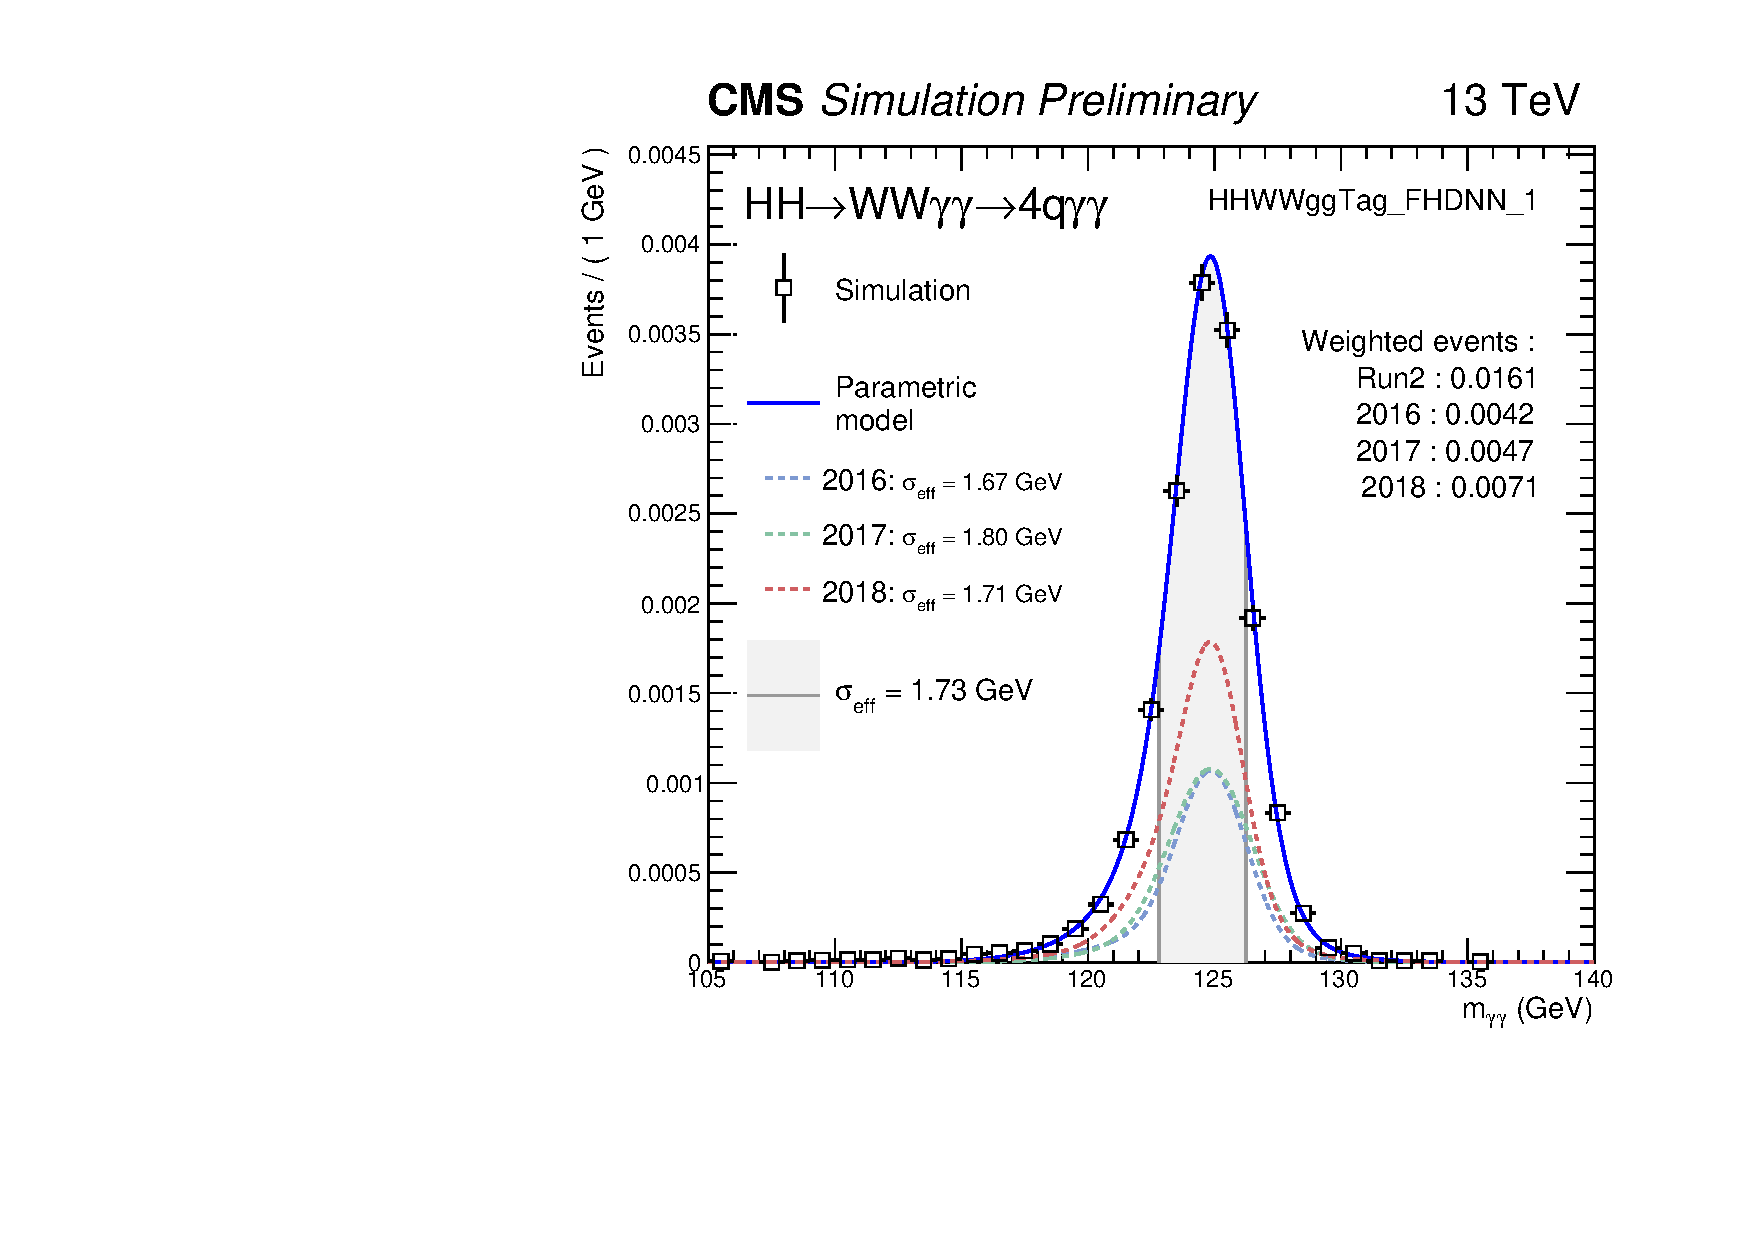
\includegraphics[width=0.75\textwidth]{Images/AnalyticFitting/Signal/smodel_HHWWggTag_FHDNN_1.pdf}
  \caption{FH signal model in the second most sensitive category}
\label{fig:FHSignalModel}
\end{figure}

\subsection{Single Higgs background}

There are expected resonant background processes present in the signal region, $115 < \mgg < 135$ GeV, due to $H\rightarrow\gamma\gamma$ processes, which cannot be modeled with a data-driven
method using data sideband events. These backgrounds are modeled with MC in the same fashion as the $HH\rightarrow WW\gamma\gamma$ signals as described in Sec. \ref{sec:SignalFitting}. The single higgs
processes considered as resonant backgrounds are the gluon-gluon fusion, vector boson fusion, associated production with a vector boson, and associated production with a top quark pair (ttH), where the Higgs boson decays 
into two photons. A separate fit is made for each analysis category and production mode. For cases in which there is a very small number of MC statistics, the diphoton shape from 
the di-Higgs signal model in the same analysis category is taken and scaled to the single higgs yield in this category, and used to model the single higgs shape in this category. 

\subsection{Continuum background}
\label{sec:AnalyticFitting_Background}

A data-driven background model is produced for each category using the data sidebands in the regions $100 < \mgg < 115$ GeV and $135 < \mgg < 180$ GeV.
The aim of this is to model the continuum background.
After the event selections and categorizations described in Sec. \ref{sec:event_selection} are applied, analytic functions are fit to the resulting $\mgg$ distributions in the data sidebands for each category.
These are later combined with their corresponding signal models in order to extract final results.
As with the signal fitting, an F-Test is performed first in order to obtain initial best-fit estimates for backgrounds functions to the data-sidebands, and to determine which functions will be considered.
Bernstein, laurent, exponential, and powerlaw function families are considered as
candidates to fit the data, and F-Tests are performed for each of these. The three data taking years are merged together before the F-test and function fitting is performed. 
After determining which functions pass the F-Test, a best fit function is chosen with the envelope method by treating the choice of function as a discrete nuisance parameter.
An uncertainty is then assigned to the chosen fit function based on a combination of the likelihoods of all attempted fit functions. This method is described in
Ref. \cite{Dauncey_2015}.

After obtaining signal models, continuum background models and Single-Higgs models for each final state, a signal plus background fit is performed.
The combination of all categories' signal plus background fits in the range 100 $<$ $\mgg$ $<$ 180 GeV, where each category is weighted by S over S$+$B, is shown in Figure \ref{fig:Run2SplusB}.

\begin{figure}[!htbp]
  \centering
  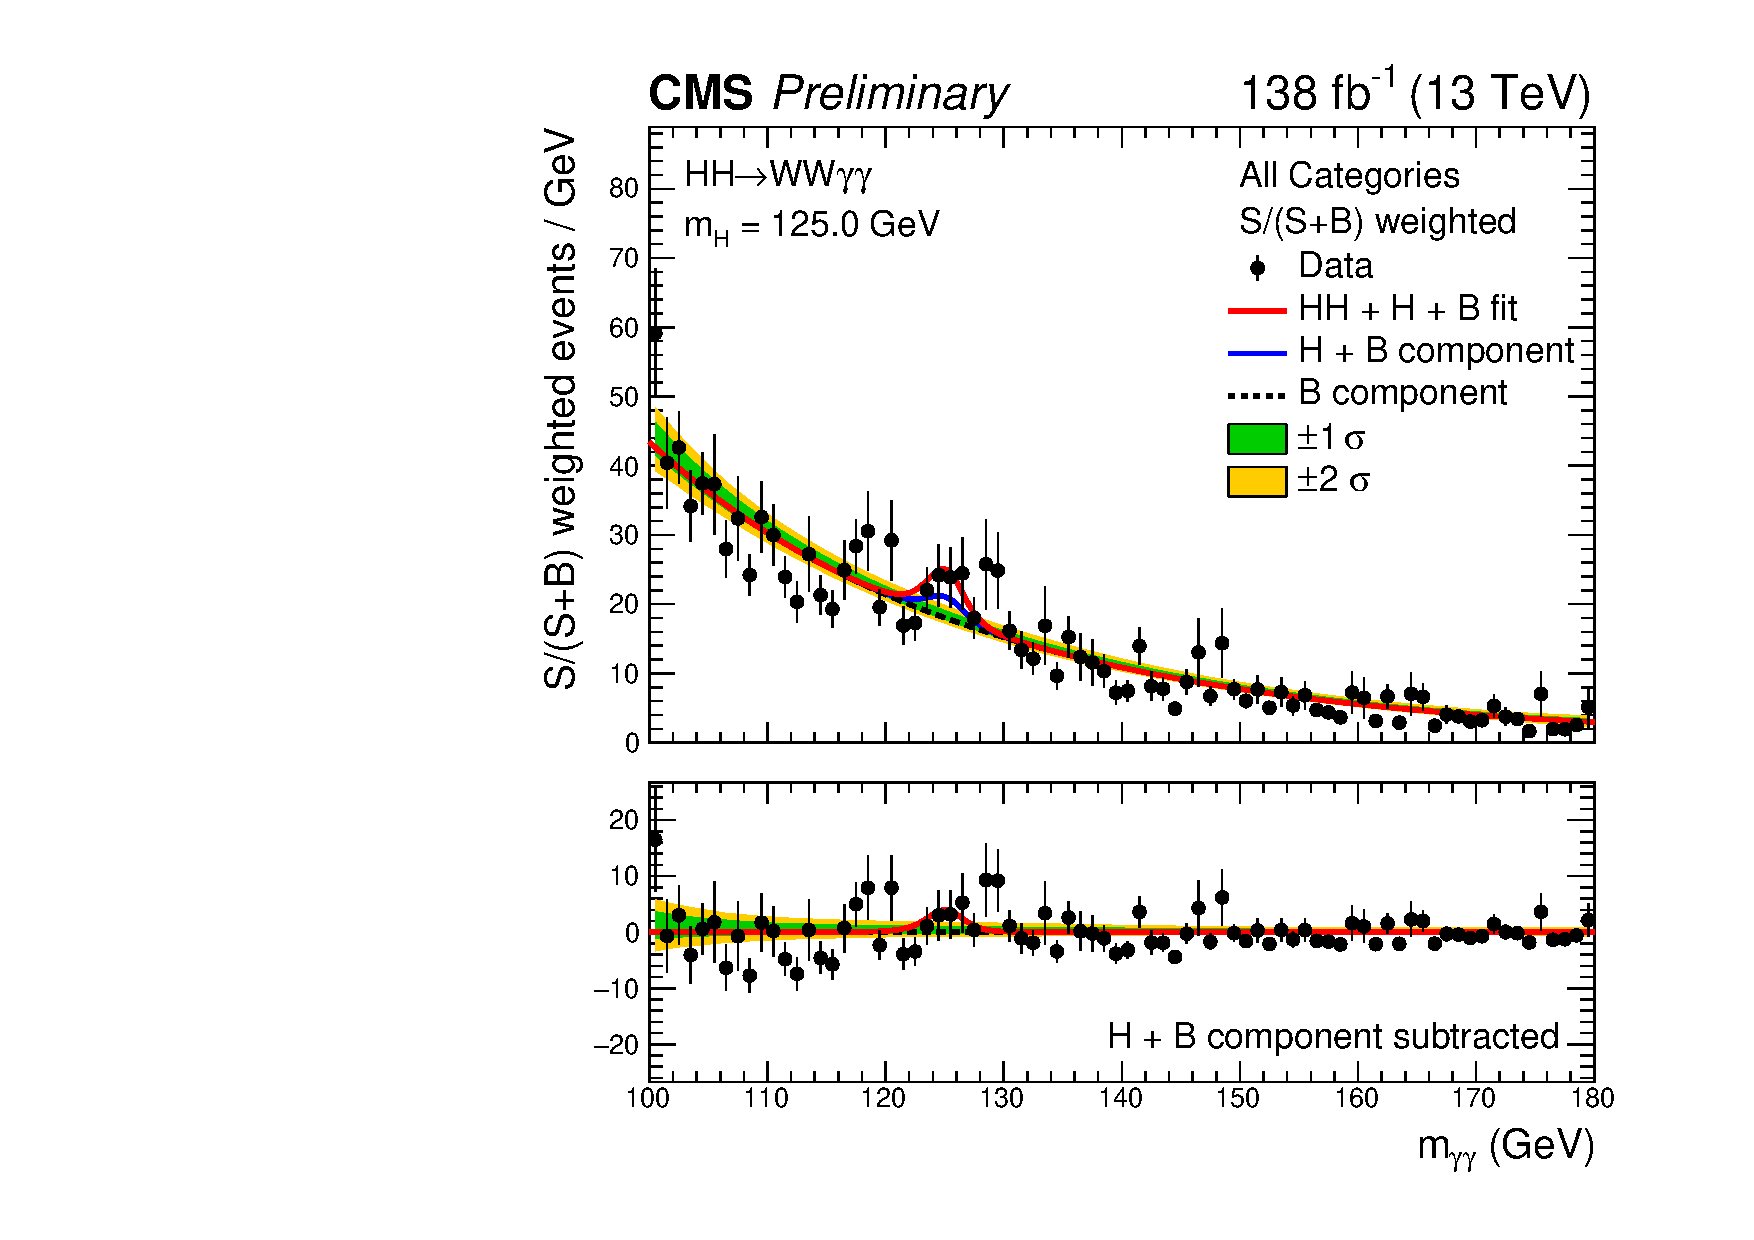
\includegraphics[width=0.9\textwidth]{Images/Results/All_combined_SplusB.pdf}
 \caption{The observed diphoton mass distribution including the signal plus background fit (red), the Single-Higgs + continuum background fit (blue) and the continuum background (black dashed line), 
 with bands covering the $\pm 1\sigma$ and $\pm 2\sigma$ uncertainties in the fitted background where all analysis categories are combined and weighted by S over S$+$B.}
  \label{fig:Run2SplusB}
\end{figure}
